Each model has its own advantages and disadvantages. Boarding by blocks allows passengers to sit according to their own preference, be it staying with their families or friends or sitting in a specific area of the airplane. This freedom makes it impossible to optimize problematic aspects such as the ones previously discussed. On the other hand, Steffen’s method is much more strict in regards to where each passenger is seated, ignoring their preference or special condition in order to reduce interference within the same three seat block. The subsequent higher efficiency was obvious in chapter 5, as the model did prove to be much more practical in sitting passengers down. However, it was also observed that in Model 1 passengers spent less time storing their luggage, which is definitely a problem that Steffen’s method ends up ignoring.

\indent\newline
This said, a third model was developed to optimize the luggage disposition inside the airplane while aiming for the unobstructed boarding sequence Model 2 excels at. The logic behind its boarding sequence can be divided into three steps:

\section{The Third Method Algorithm}
\subsection{Step 1: Assigning the passengers to a specific seat according to their luggage quantity}
This is a pre-boarding step. All passengers are distributed by the seats according to the quantity of luggage they have, in order to have the passengers with less luggage seated closer to the windows, and the passengers with more luggage seated closer to the aisle. This is because the less luggage they have, the less time they spend storing it and consequently the smaller the chances another passenger will arrive in the meantime and wait in the aisle. Once seated in their seats, passengers seated near the window won't need anything else. 

\indent\newline
The order of the quantity of luggage entering the airplane will then be: 0, 0, 0, 0, 0, 0, 0, 0, 0, 0, 0, 0, 0, 0, 0, 0, 0, 0, 0, 1, 1, 1, 1, 1, 1, 1, 1, 1, 1, 1, 1, 1, 1, 1, 1, 1, 1, 1, 1, 1, 1, 1, 1, 1, 1, 1, 1, 1, 1, 1, 1, 1, 1, 1, 1, 1, 1, 1, 1, 1, 1, 1, 1, 1, 1, 1, 1, 1, 1, 1, 1, 1, 1, 1, 1, 1, 1, 1, 1, 1, 1, 1, 1, 1, 1, 1, 1, 1, 1, 1, 1, 1, 1, 1, 1, 1, 1, 1, 1, 2, 2, 2, 2, 2, 2, 2, 2, 2, 2, 2, 2, 2, 2, 2, 2, 2, 2, 2, 2, 2. The following table shows the quantity of luggage associated to each one of the 120 seats:
\begin{table}[H]
  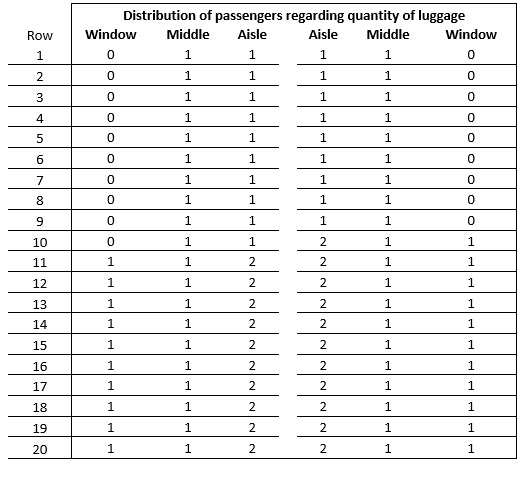
\includegraphics[width=0.75\textwidth]{tables/luggage.jpg}
  \caption{Luggage Distribution}
  \label{tbl:luggage}
\end{table}
\subsection{Step 2: Optimization}
This is also a pre-boarding step that tries to optimize the sequence defined in step 1, avoiding the need for passengers to change the bin as much as possible. The algorithm loops through the bins to simulate the luggage distribution inside the airplane and does the following:
\indent \newline
\begin{itemize}
\item If the bin's capacity is exceeded by 2 or more luggages, check if it's possible to change a passenger with 2 luggages that would be seated under this bin by a passenger with 0 luggage seated under a different bin with at least 2 available places.
\item If the bin's capacity is exceeded by just 1 luggage, check if it's possible to change  a passenger with 1 luggage that would be seated under this bin by a passenger with 0 luggage seated under a different bin with at least 1 available place
\item Update the boarding sequence of passengers 
\item Stop if no more passengers can be swapped.
\end{itemize}

\indent \newline
Some important observations about this step: since the algorithm's priority is to avoid the passengers need to change their respective bins, it is possible to change a passenger with luggage in an aisle seat with a passenger without luggage in a window seat. Also, a passenger will only change bin if it is possible to store all of his luggage in the candidate bin. 

\subsection{Step 3 Ordering the passengers according to Steffen’s Method}
After the arrangements in steps 1 and 2, the passengers will board according to the proposed method of Steffen.

\section{Improvements}
In order to check whether this new model is indeed an improvement from the previous two, the same performance metrics were used and the same passenger data set ("PassengersNormal") was chosen. By looking at the table below, it can be noticed that even though Model 3 did not differ much from Model 2 regarding the pre-boarding time and the waiting time to show documentation at the end of the queue, it succeeded in minimizing the time passengers spend storing their luggage, consequently reducing the total boarding time. This is also indicated by the percentage of passengers that end up using a bin other than the one above their seat, which was reduced from 15\% to 0\%, meaning that every passenger was able to store their belongings in their respective bin.


\begin{table}[H]
  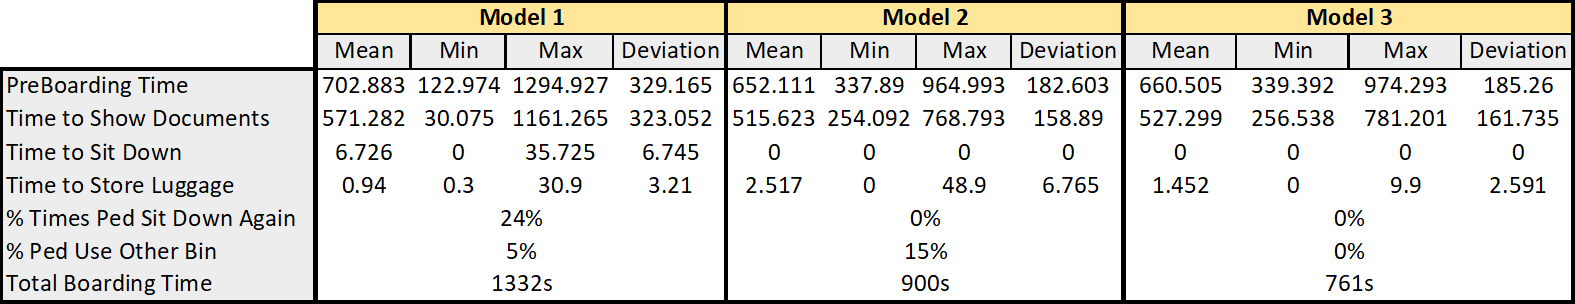
\includegraphics[width=1.0\textwidth]{tables/statistics2.png}
  \caption{Time Statistics - Model 3}
  \label{tbl:statistics2}
\end{table}
